\documentclass[12pt]{article}
\usepackage[a4paper, margin=0.75in]{geometry}
\usepackage[document]{ragged2e}
\usepackage{graphicx}
\usepackage{placeins}
\graphicspath{ {./images/} }
\usepackage{enumerate}
\usepackage{framed}
\usepackage{amsmath,amsfonts,amsthm,thmtools,amssymb,mathtools,commath}
\usepackage{physics}
\usepackage{tikz}
\usetikzlibrary{mindmap}
\usepackage{caption}
\usepackage{xcolor}
\usepackage[most]{tcolorbox}
\usepackage{cleveref}


%%%%%%%%%%%%%%%%
%  Definition  %
%%%%%%%%%%%%%%%%
\tcbuselibrary{theorems,skins,hooks}
\newtcbtheorem[number within=subsection]{definition}{Definition}%
{
    % theorem style=definition,
    enhanced,
	before skip=2mm,after skip=2mm, colback=cyan!5,colframe=cyan!80!black,boxrule=0.5mm,
	attach boxed title to top left={xshift=1cm,yshift*=1mm-\tcboxedtitleheight},
	boxed title style={frame code={
					\path[fill=cyan]
					([yshift=-1mm,xshift=-1mm]frame.north west)
					arc[start angle=0,end angle=180,radius=1mm]
					([yshift=-1mm,xshift=1mm]frame.north east)
					arc[start angle=180,end angle=0,radius=1mm];
					\path[left color=cyan!30!black,right color=cyan!30!black,
						middle color=cyan!50!black]
					([xshift=-2mm]frame.north west) -- ([xshift=2mm]frame.north east)
					[rounded corners=1mm]-- ([xshift=1mm,yshift=-1mm]frame.north east)
					-- (frame.south east) -- (frame.south west)
					-- ([xshift=-1mm,yshift=-1mm]frame.north west)
					[sharp corners]-- cycle;
				},interior engine=empty,
		},
	fonttitle=\bfseries,
	title={#2},#1
}{def}


%%%%%%%%%%%%%
%  Theorem  %
%%%%%%%%%%%%%
\tcbuselibrary{theorems,skins,hooks}
\newtcbtheorem[use counter from=definition]{theorem}{Theorem}%
{
    theorem style=plain,
    enhanced,
    colframe=green,
    boxrule=1pt,
    titlerule=0mm,
    toptitle=1mm,
    bottomtitle=1mm,
    fonttitle=\bfseries,
    fontupper=\mdseries\itshape,
    coltitle=green!30!black,
    colbacktitle=cyan!15!white,
    colback=green!10,
    description font=\bfseries\sffamily
}{thrm}


%%%%%%%%%%%%%%
% Corollary  %
%%%%%%%%%%%%%%
 \tcbuselibrary{theorems,skins}
 \newtcbtheorem[use counter from=theorem]{corollary}{Corollary}%
 {
    theorem style=plain,
    enhanced,
    colframe=green,
    frame hidden,
    titlerule=0mm,
    toptitle=1mm,
    bottomtitle=1mm,
    fonttitle=\bfseries,
    fontupper=\mdseries\itshape,
    coltitle=green!30!black,
    colbacktitle=cyan!15!white,
    colback=green!10,
    description font=\bfseries\sffamily
 }{corl}


%%%%%%%%%%%%%
%  Example  %
%%%%%%%%%%%%%
\tcbuselibrary{theorems,skins,hooks}
\newtcbtheorem[number within=section]{example}{Example}%
{
	enhanced,
	breakable,
	colback = gray!5,
	frame hidden,
	boxrule = 0sp,
	borderline west = {2pt}{0pt}{gray},
	sharp corners,
	detach title,
	before upper = \tcbtitle\par\smallskip,
    coltitle=gray!70!black,
	fonttitle = \bfseries\sffamily,
	description font = \mdseries\bfseries
}
{xmp}


%%%%%%%%%%%%%%
%  Exercise  %
%%%%%%%%%%%%%%
\tcbuselibrary{theorems,skins,hooks}
\newtcbtheorem[number within=section]{exercise}{Exercise}%
{
    enhanced,
    breakable,
    colback=black!5,
    colframe=black!30,
    left=0.5em,
    before skip=10pt,
    after skip=10pt,
    boxrule=0pt,
    boxsep=0pt,
    arc=0pt,
    outer arc=0pt,
    borderline west={3pt}{0pt}{black!30},
}{exc}

%%%%%%%%%%
%  Note  %
%%%%%%%%%%
\usetikzlibrary{arrows,calc,shadows.blur}
\tcbuselibrary{skins}
\newtcolorbox{note}[1][]{%
	enhanced jigsaw,
	colback=gray!20!white,%
	colframe=gray!80!black,
	size=small,
	boxrule=1pt,
	title=\textbf{Note:-},
	halign title=flush center,
	coltitle=black,
	breakable,
	drop shadow=black!50!white,
	attach boxed title to top left={xshift=1cm,yshift=-\tcboxedtitleheight/2,yshifttext=-\tcboxedtitleheight/2},
	minipage boxed title=1.5cm,
	boxed title style={%
			colback=white,
			size=fbox,
			boxrule=1pt,
			boxsep=2pt,
			underlay={%
					\coordinate (dotA) at ($(interior.west) + (-0.5pt,0)$);
					\coordinate (dotB) at ($(interior.east) + (0.5pt,0)$);
					\begin{scope}
						\clip (interior.north west) rectangle ([xshift=3ex]interior.east);
						\filldraw [white, blur shadow={shadow opacity=60, shadow yshift=-.75ex}, rounded corners=2pt] (interior.north west) rectangle (interior.south east);
					\end{scope}
					\begin{scope}[gray!80!black]
						\fill (dotA) circle (2pt);
						\fill (dotB) circle (2pt);
					\end{scope}
				},
		},
	#1,
}


\title{
    CSE-284: Object Oriented Programming \\
    Experiment 1: Introduction to Class and Objects in OOP
}

\author{
    Turja Roy \\ 
    ID: 2108052 \\ 
    Group: G-2
}
\date{}

\begin{document}
\maketitle

\section*{Objectives:}
\begin{itemize}
    \item Introduction with Classes and Objects in C++. 
    \item To create data member and member functions (Methods) in a class. 
    \item To understand the concept of visibility of data member and member functions (Public and Private access).
\end{itemize}


\FloatBarrier
\section*{Example 1}
Write a C++ program to define a class \texttt{Box} and create objects of this class.

\subsection*{Code}
\lstinputlisting[language=C++]{../Exp-1.cpp}

\subsection*{Output}
\begin{figure}[htpb]
    \centering
    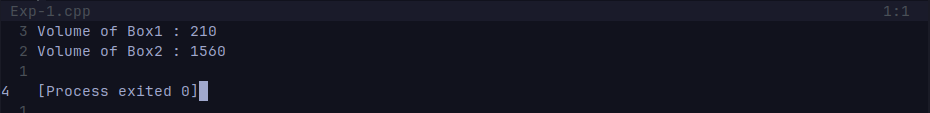
\includegraphics[width=0.8\textwidth]{Exp-1.png}
    \caption{Output of Exp-1.cpp}
\end{figure}


\FloatBarrier
\section*{Example 2}
Write a C++ program to define a class \texttt{Box} with member functions.

\subsection*{Code}
\lstinputlisting[language=C++]{../Exp-2.cpp}

\subsection*{Output}
\begin{figure}[htpb]
    \centering
    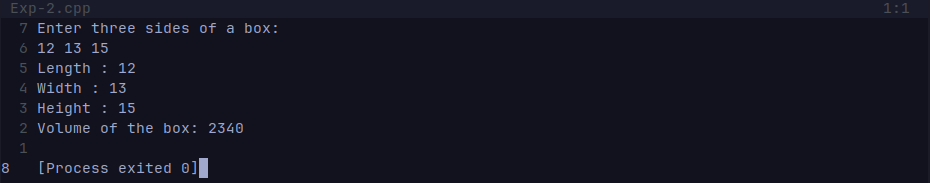
\includegraphics[width=0.8\textwidth]{Exp-2.png}
    \caption{Output of Exp-2.cpp}
\end{figure}


\FloatBarrier
\section*{Example 3}
Write a C++ program to define a class \texttt{Box} with member functions.

\subsection*{Code}
\lstinputlisting[language=C++]{../Exp-3.cpp}

\subsection*{Output}
\begin{figure}[htpb]
    \centering
    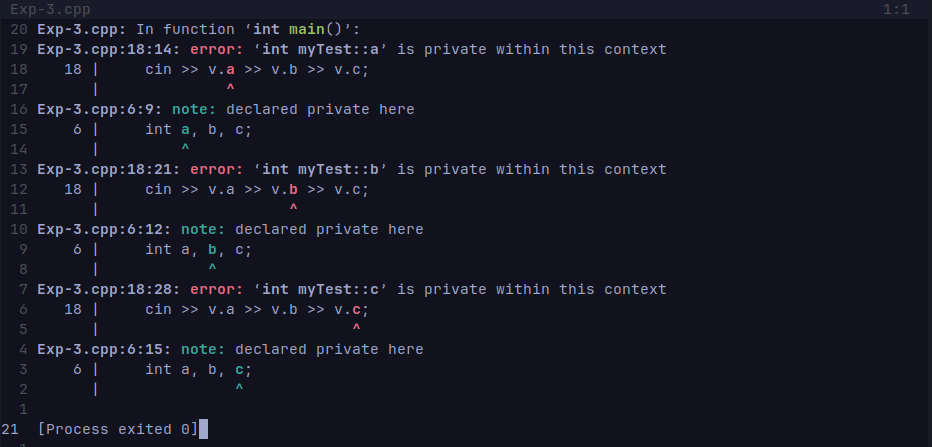
\includegraphics[width=0.7\textwidth]{Exp-3-Error.png}
    \caption{Exp-3 error log}
\end{figure}
\begin{figure}[htpb]
    \centering
    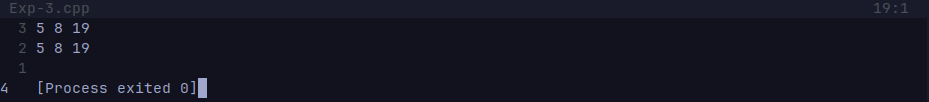
\includegraphics[width=0.8\textwidth]{Exp-3-Error-fixed.png}
    \caption{Output of Exp-3.cpp After fixing error}
\end{figure}


\FloatBarrier
\section*{Example 4}
Write a C++ program to understand public and private access of class members.

\subsection*{Code}
\lstinputlisting[language=C++]{../Exp-4.cpp}

\subsection*{Output}
\begin{figure}[htpb]
    \centering
    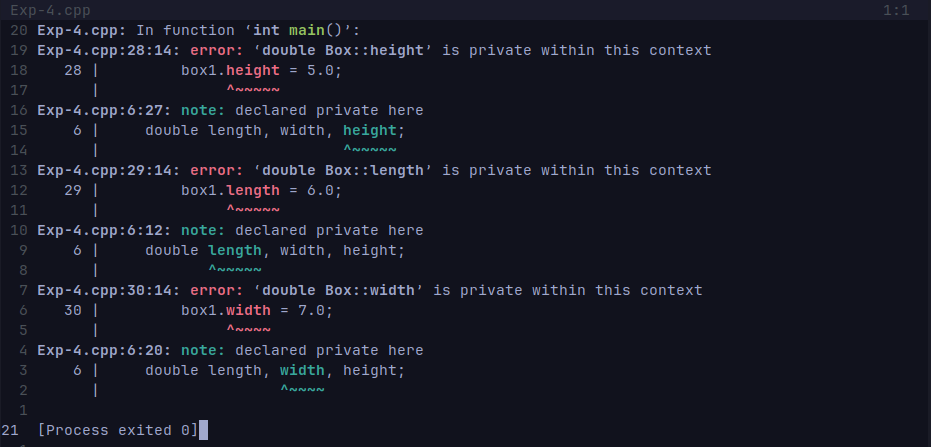
\includegraphics[width=0.7\textwidth]{Exp-4-Error.png}
    \caption{Exp-4 error log}
\end{figure}
\begin{figure}[htpb]
    \centering
    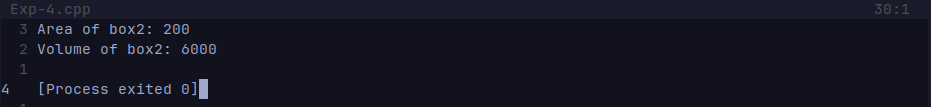
\includegraphics[width=0.8\textwidth]{Exp-4-Error-fixed.png}
    \caption{Output of Exp-4.cpp After fixing error}
\end{figure}


\FloatBarrier
\section*{Lab Task}
Write a C++ program to calculate the CGPA of a student using class and objects.

\subsection*{Code}
\lstinputlisting[language=C++]{../Lab-Test.cpp}

\subsection*{Output}
\begin{figure}[htpb]
    \centering
    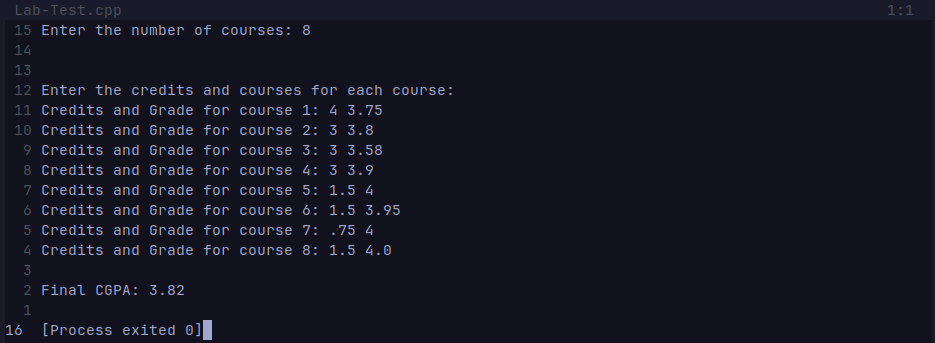
\includegraphics[width=0.8\textwidth]{Lab-Test.png}
    \caption{Output of CGPA Calculator}
\end{figure}


\FloatBarrier
\section*{Practice Exercise 1}
Write a class having two private variables and one member function which will return the area and parimeter of the rectangle. 

\subsection*{Code}
\lstinputlisting[language=C++]{../Prac-1.cpp}

\subsection*{Output}
\begin{figure}[htpb]
    \centering
    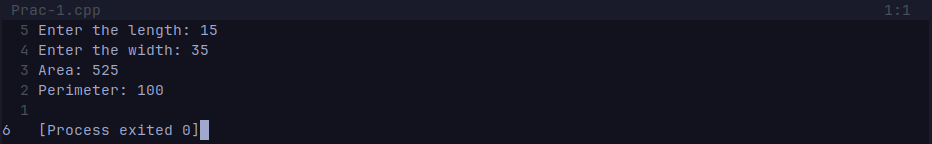
\includegraphics[width=0.8\textwidth]{Prac-1.png}
    \caption{Output of Prac-1.cpp}
\end{figure}


\FloatBarrier
\section*{Practice Exercise 2}
Write a C++ program to define a class \texttt{batsman} with the following specifications:
\begin{itemize}
    \item Private members:
    \begin{itemize}
        \item \texttt{batsman\_code}: 4 digits code number
        \item \texttt{batsman\_name} 20 characters (string)
        \item \texttt{total\_innings, notout\_innings, total\_runs}: integer type
        \item \texttt{calcavg()}: Function to compute batavg
    \end{itemize}
    \item Public members:
    \begin{itemize}
        \item \texttt{readdata()}: Function to accept value from batsman code, batsman name, to- tal innings, notout innings, total runs and invoke the function calcavg().
        \item \texttt{displaydata()}: Function to display the data members on the screen.
    \end{itemize}
\end{itemize}

\subsection*{Code}
\lstinputlisting[language=C++]{../Prac-2.cpp}

\subsection*{Output}
\begin{figure}[htpb]
    \centering
    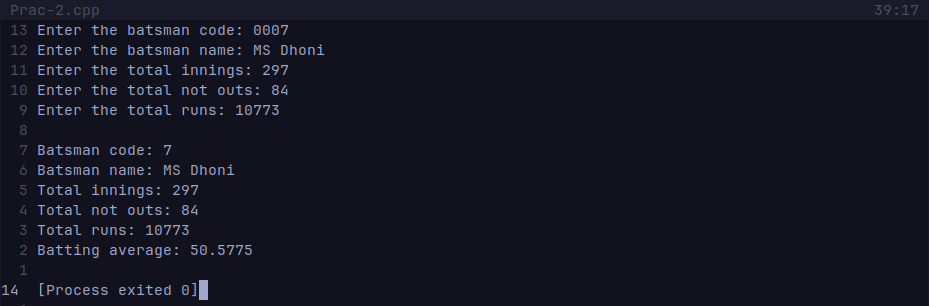
\includegraphics[width=0.8\textwidth]{Prac-2.png}
    \caption{Output of Prac-2.cpp}
\end{figure}


\newpage
\section*{Discussion}
\begin{itemize}
    \item In this lab, basic concepts of class and objects in C++ were discussed.
    \item The visibility of data members and member functions were discussed.
    \item When a private member is accessed from outside the class, it generates an error. The errors can be fixed by making the member public, or by using public member functions.
\end{itemize}

\end{document}
